\section{Visual System}
To have a wide field of view and a small image size we use log-polar images \cite{sandini80retinalike}. They mimic the photoreceptors distribution in the retina and the topological trasform from the retina to the visual cortex. In these images we have only a small center area with a high resolution (fovea) while in the periphery the resolution decrease exponentially moving away from the center. Like in humans, there is the need to move the sensor to take high resolution snapshots of important points in the scene, according to a given task or simple to quickly gather information about the scene. That is there is the need to have a system to select information points and to deeply analyze them.

To precisely manipulate an object the robot must be able to segment a scene in objects, in particular to segment an object from its background. It is not enough to poorly localize the object, we need a segmentation of the object to derive its spatial position. This is thightly coupled with the problem of defining what an object is, that is to define what are the properties of ``objecthood''.

What we propose is not to define what an object is, but to use the definition of ``proto-objects''. They are a step above the mere features, possessing some but not all the caracteristics of an object; clusters of points on the image ``naturally'' grouped together. The idea of proto-objects has its roots in psycological literature [cite], but also in the neurobiological one. In fact it has been proposed that the synchronization of visual cortical neurons can be the carrier of the perceptual grouping phenomenon \cite{eckhorn88coherent,gray89oscillatory}. We propose the use of the watershed transform (rainfalling variant) \cite{smet00rainfalling} on the edge map of a feature extraction stage to simulate the results of the synchronization. In this way the image is segmented in region of constant color or with a constant gradient of color (blobs). A segmentation of this type as been demonstrated to happen in humans before the attention is deployed to the scene \cite{driver00segmentation}.

Our idea is that the identity of an object can not be known without any manipulation. So using actions, the robot can go beyond the concepts of proto-objects, learning a model of an object. In particular an object is seen as a collection of proto-objects and their spatial relations. In pratice manipulating an object the system can acquire different views of it, and, using the probabilities of occurrence, calculate the probability the collection of blobs fixed at a given moment is the object it is searching for. Then, using these same probabilities, a figure-ground segmentation can be attempted. More details about this model can be found in \cite{orabona05object}.

The segmentation is then used as a mask to the stereo algorithm. In this way we can save time not calculating the depth map on all the image, and, defining a region of interest around the object, you can calculate the local orientation in the space and use this information to guide different behaviors from the robot.

In order to achieve a good detection of the object orientation, we had to develop a fast and robust stereo algorithm, which was able to work in real world conditions.

The algorithm is mainly based on the work by Van Meerbergen et al. \cite{merrbergen02stereo}, where, given a scanline, all the possible matches between pixels are investigated by exploring a graph (using the dynamic programming) built by assigning a cost to each position pair and to each occlusion. The algorithm works very well and it is fast enough, especially when handling small images. But few problems arose: typically our environment consists in one or more objects of interest which are very close, compared to the interocular distance, to the robot. The consequence is that a surface can be very different in shape between the two images of the stereo pair. So we had to slightly modify the original algorithm. In order to solve the former problem, we decided to relax one constraint: a pixel is now allowed to belong to two (or even more) matches in the same match sequence. The result is that a short sequence of pixel in one image can match a long one in the other image of the pair. 

Since the complexity, for each graph (i.e. each scanline) of dynamic programming is $O(m)$ (where $m$ is the total number of arcs in the graph and it is proportional to the length of the scanlines), we consider only the portion of the image around the object of interest, segmenting the object itself by using the information coming from the saliency algorithm. This reduces both m and the number of  lines to be processed.
We added another additional step: once computed the disparity map $D_{l-r}$ (displacement of the pixels in the left image compared to the ones in the right one), we use its information to detect the object position on the right image, according to the formula: 
\begin{equation}D_{l-r}(x)=D_{r-l}(x-D_{l-r}(x))\end{equation}

This result will be used to segment the object on the right image. The images are then swapped and the disparity is computed again. This new result will be used to validate and correct the previous one.

\begin{figure}
\centering
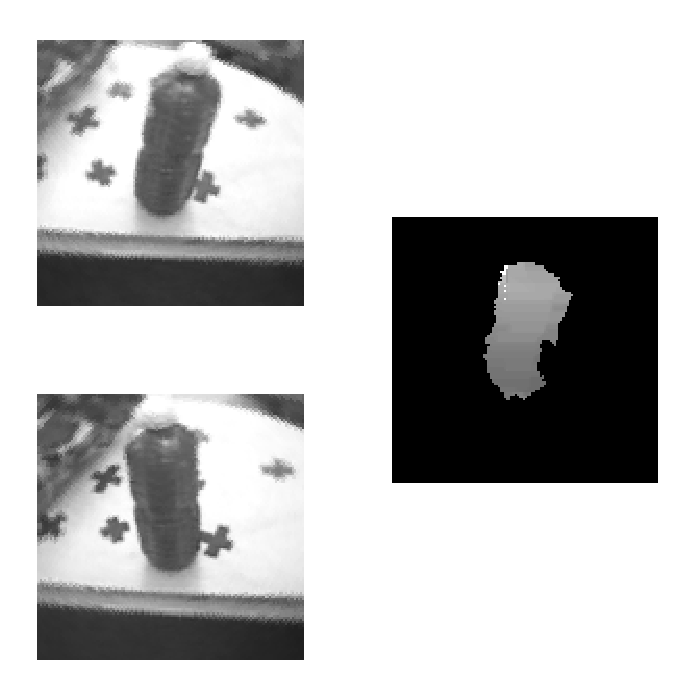
\includegraphics[width=3in]{disparity}
\caption{The Disparity Algorithm  Left: The Stereo Pair, Right: The Final Disparity Map, masked. The mask image comes from the attention algorithm.}
\label{disparity}
\end{figure}
